\documentclass[]{jsarticle}
\usepackage[dvipdfmx]{graphicx}
\usepackage{ascmac}
\AtBeginDocument{\RequirePackage{lmodern, times}}
\usepackage{ulem}
%%%%%%%%%%%%%%%%%
\usepackage{here}
\usepackage{txfonts}
\usepackage{listings, jlisting}
\renewcommand{\lstlistingname}{プログラム}
\lstset{language=C,
  basicstyle=\ttfamily\scriptsize,
  commentstyle=\textit,
  classoffset=1,
  keywordstyle=\bfseries,
  frame=tRBl,
  framesep=5pt,
  showstringspaces=false,
  numbers=left,
  stepnumber=1,
  numberstyle=\tiny,
  tabsize=2
}
%%%%%%%%%%%%%%%%%
\usepackage{circuitikz}


\begin{document}
\title{2SK2936のテスト}
\author{青木翔平}
\date{29, Jul 2015}
\maketitle

\section{テストベンチ}
\subsection{回路図}
\sout{テスト時の回路図を図\ref{testbench}に示す}。
図は間違い。プローブのGNDはGNDに、プローブは抵抗とMOSFETのドレイン間につなぐ。


%\begin{figure}[htbp]
%\centering
%\begin{circuitikz}
%  \draw (0,0)
%  to[V,v=$Vcc$] (0,2)
%  to[short] (2,2)
%  to[R=$R_{1}$] (2,0)
%  to[short] (0,0);
%\end{circuitikz}
%\caption{動作試験回路}
%\label{testbench}
%\end{figure}


\begin{figure}[htbp]
\centering
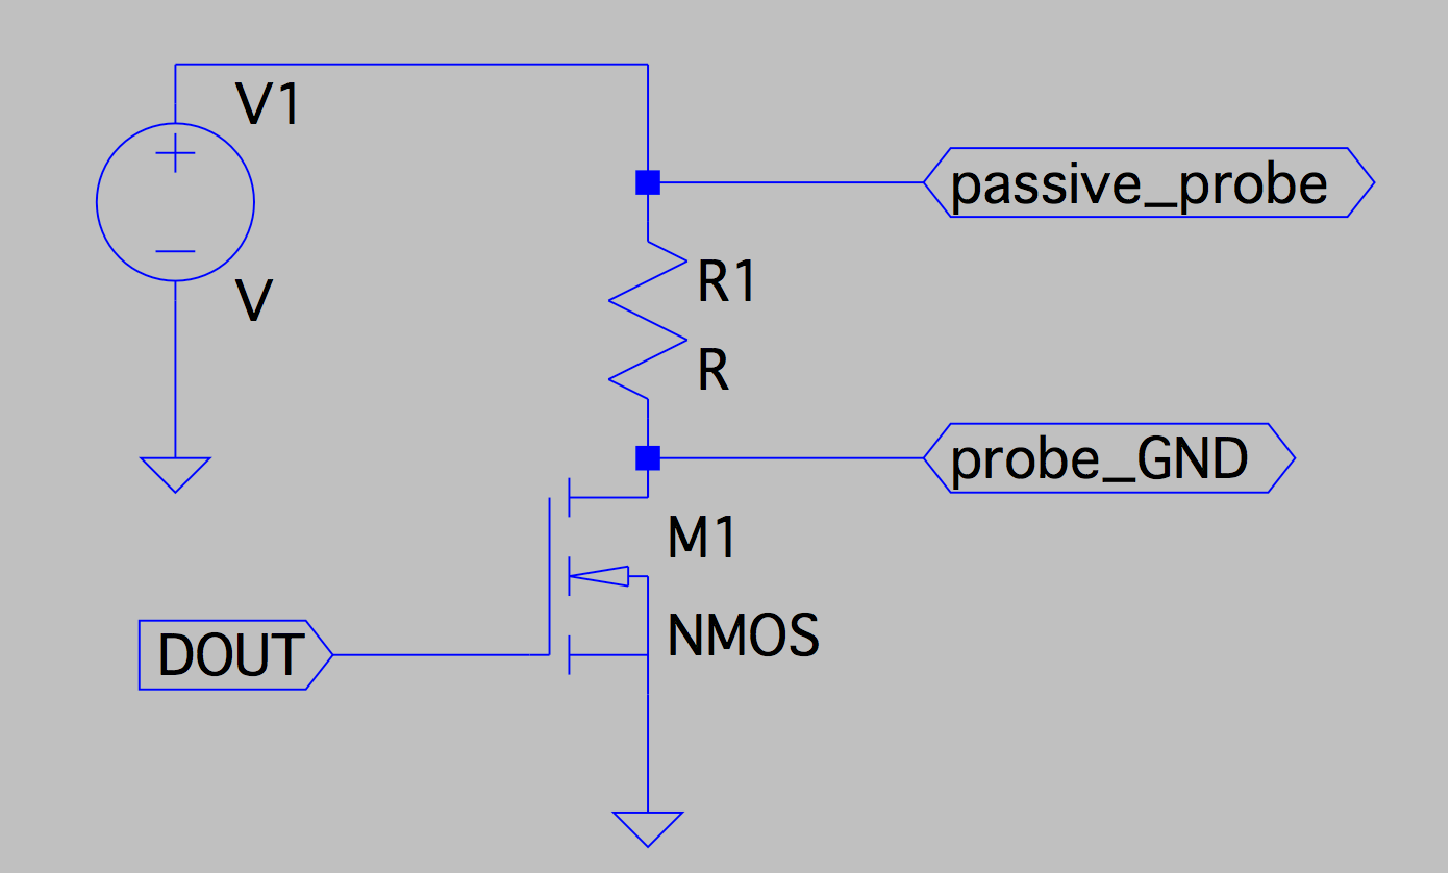
\includegraphics[width=130mm]{./image/testbench.pdf}
\caption{動作試験回路}
\label{testbench}
\end{figure}

\subsection{抵抗値計算}
試しにR=1k$\Omega$とした。この場合の抵抗での電流は、
\begin{eqnarray*}
I & = &  \frac{V}{R} \\
   & = & \frac{24}{1000} \\
   & = & 24 [mA]
\end{eqnarray*}
実際にはフォトカプラ入力電流を考慮する必要があるが、後述するスピンドルコントローラでは内部回路として抵抗を有している。したがって純粋に電圧を入力すればよく、すなわちテスト回路で用いた抵抗は省略して構わないと考えられる。

回路での消費電力は
\begin{eqnarray*}
W & = &  I^{2} R \\
            & = & 0.024^{2} \times 1.0 \cdot 10^{3} \\
            & = & 0.576 [W]
\end{eqnarray*}
この場合1/2抵抗以上を使う必要がある。

\subsection{Arduinoスケッチ}
プログラム\ref{switch_mosfet}に用いたスケッチを示す。
はじめPWM出力をしていたが、必要ないのでデジタル出力に変更した。
\begin{lstlisting}[caption=MOSFET駆動スケッチ,label=switch_mosfet]
void setup(){
 pinMode(8,OUTPUT); 
 Serial.begin(9600);
}

void loop(){
  Serial.println("ON");
  //analogWrite(9,255);
  digitalWrite(8,HIGH);
  delay(5000);
  Serial.println("OFF");
  //analogWrite(9,0);
  digitalWrite(8,LOW);
  delay(5000);  
}
\end{lstlisting}

\subsection{オシロスコープでの確認}
オシロスコープで電圧波形を確認したところ、問題なく抵抗後の電圧が24Vを出力していた。

\section{スピンドルコントローラMT01CPとの接続}
スピンドルコントローラとの接続においては、上述のようにテスト用に配置した電気抵抗を削除して、図\ref{controller}の様に配線する。
\begin{figure}[htbp]
\centering
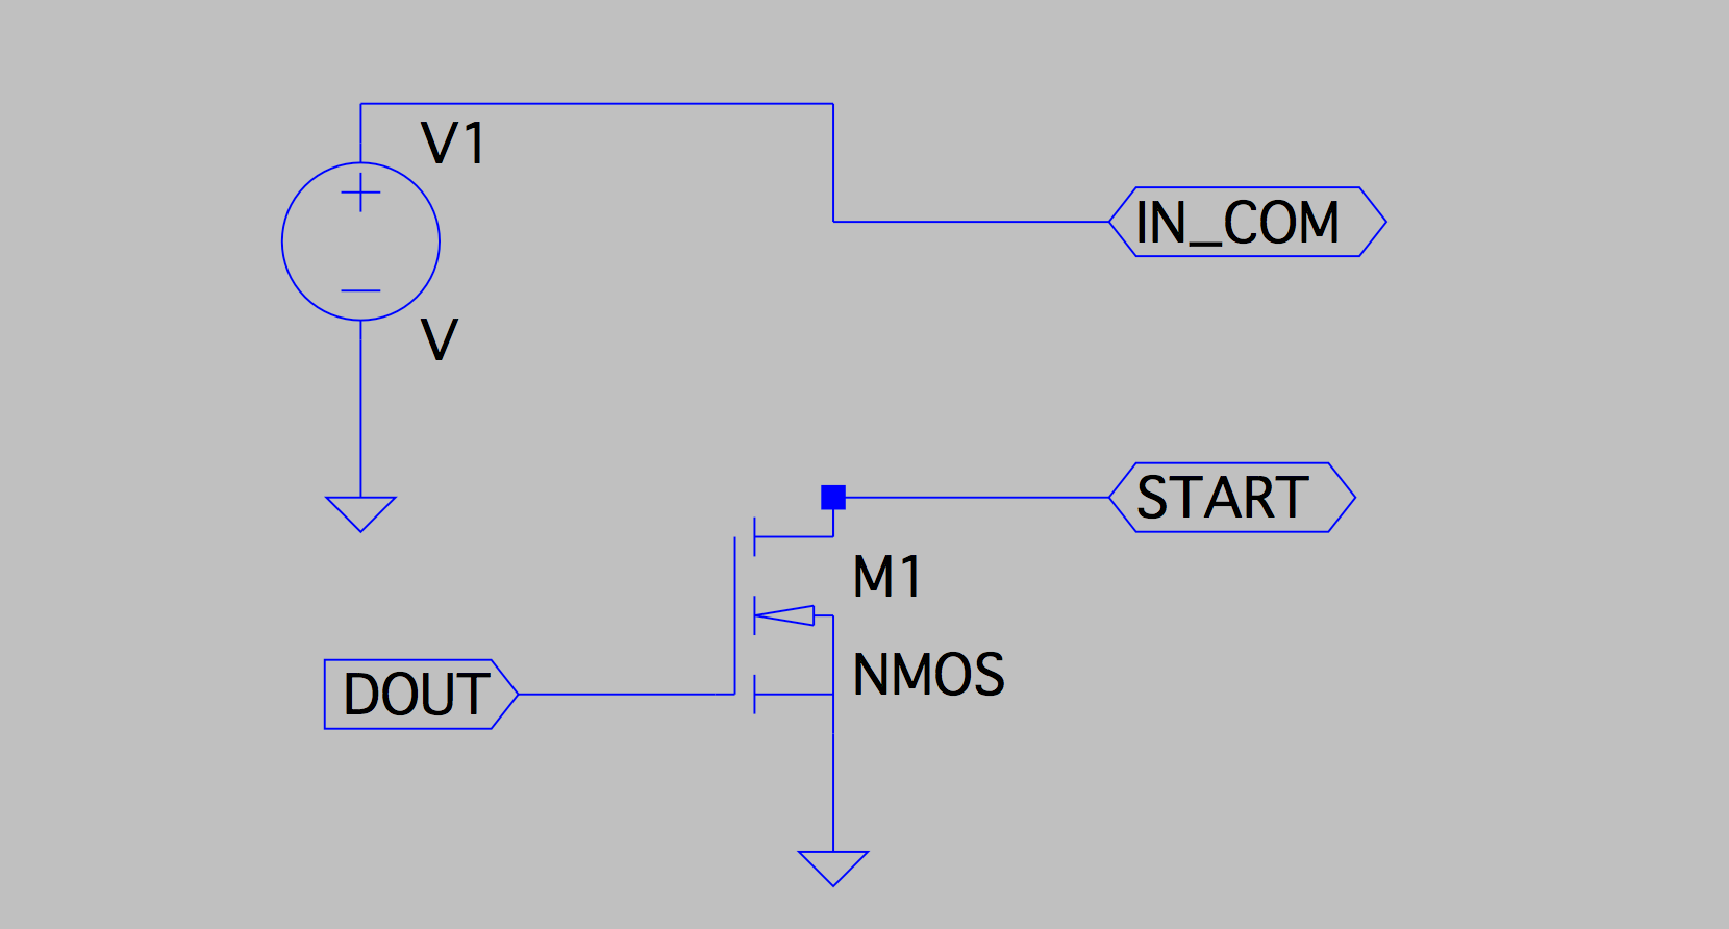
\includegraphics[width=130mm]{./image/controller.pdf}
\caption{スピンドルとの接続回路}
\label{controller}
\end{figure}

参考にコントローラの回路図を図\ref{input}に示す。フォトカプラと抵抗が接続していることがわかり、この抵抗は電流制限抵抗であると考えられる。
\begin{figure}[htbp]
\centering
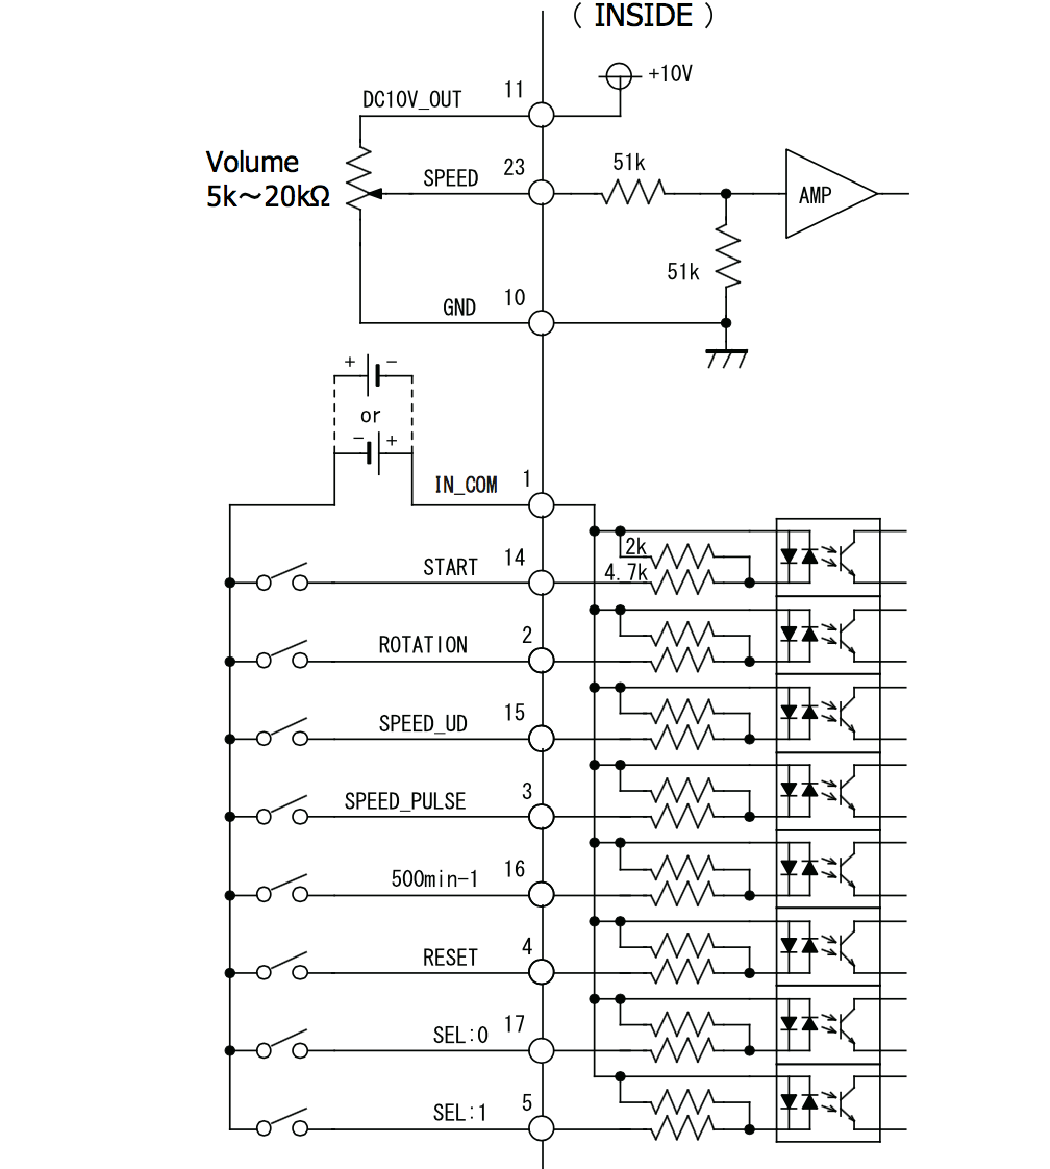
\includegraphics[width=130mm]{./image/minitor_input.pdf}
\caption{コントローラ側外部入力信号接続回路}
\label{input}
\end{figure}


%\section{オシロスコープでの出力波形計測}

%\begin{figure}[htbp]
%\centering
%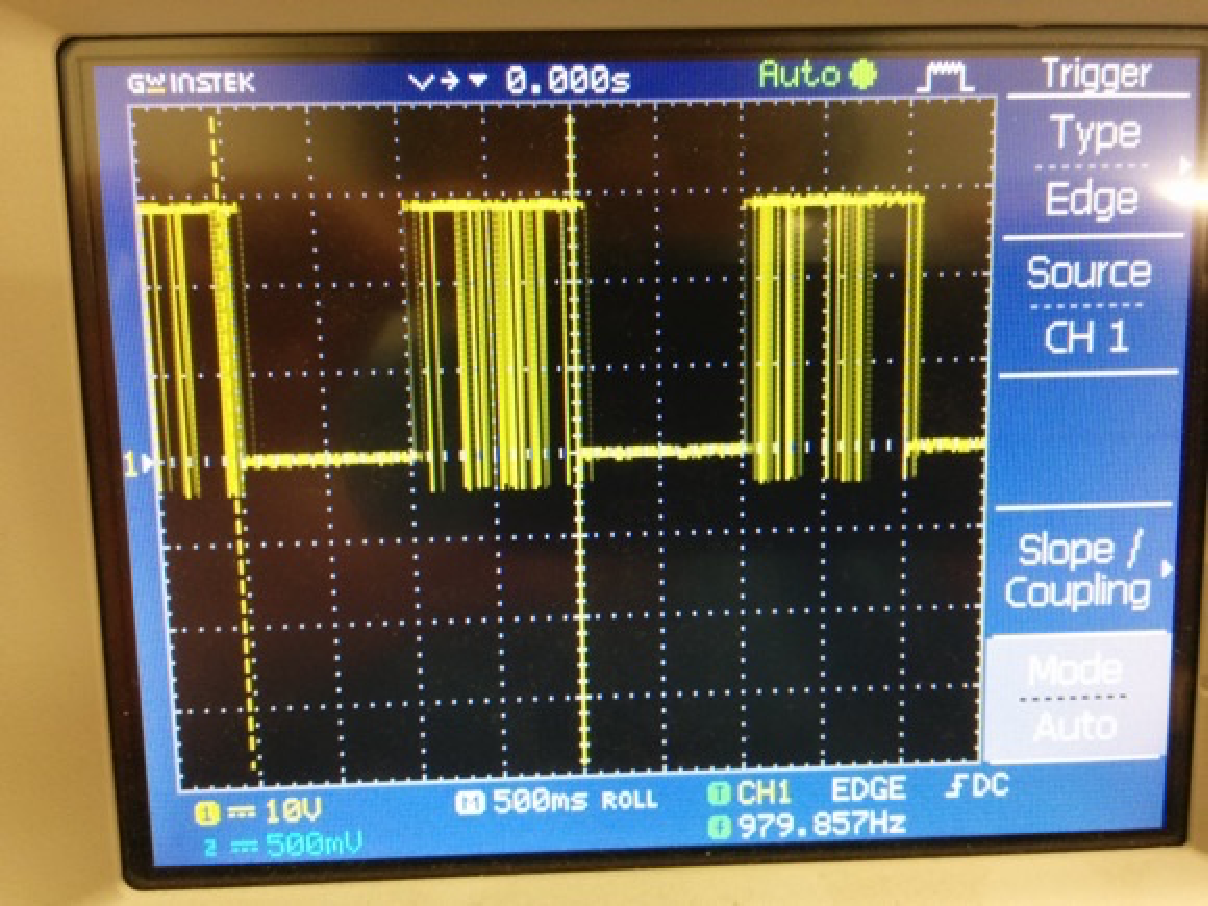
\includegraphics[width=110mm]{./image/out.pdf}
%\caption{2SK2936からの出力}
%\label{output}
%\end{figure}
%
%\begin{figure}[htbp]
%\centering
%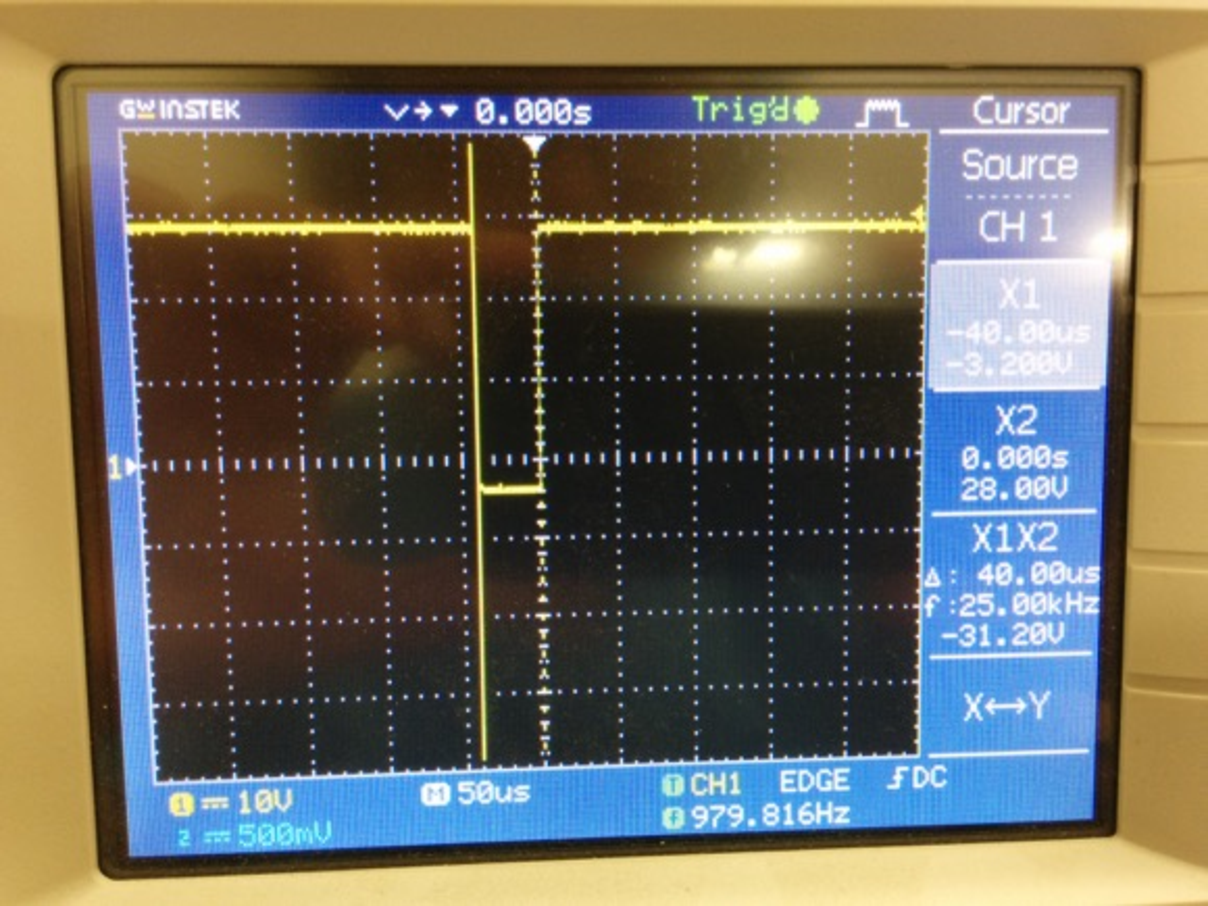
\includegraphics[width=110mm]{./image/short.pdf}
%\caption{間欠ノイズの幅=40$\mu$s}
%\label{short}
%\end{figure}
%
%\begin{figure}[htbp]
%\centering
%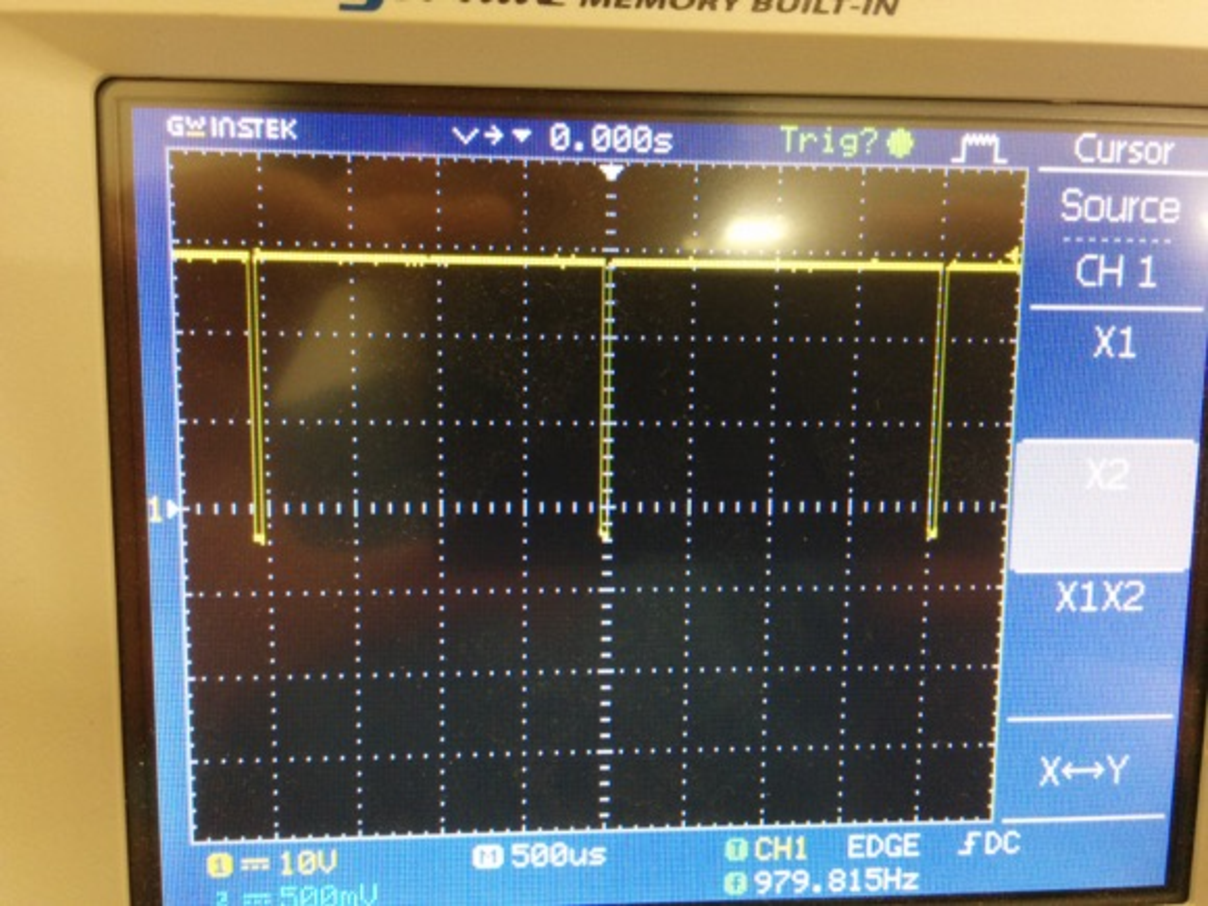
\includegraphics[width=110mm]{./image/long.pdf}
%\caption{デューティ幅=2ms}
%\label{long}
%\end{figure}




\section{備考}
\begin{itemize}
\item Arduino一台が発熱で異常な挙動を示した。
 \begin{itemize}
   \item 具体的にはPWM用に使っていた8ピンからの出力が1.8V程度しか出なくなった
 \end{itemize}
\item エジソンプラザで買ったMOSFETは使えるのか
\end{itemize}



\end{document}
